\documentclass[11pt]{article}

\def\chapitre{16}
\def\pagetitle{Relations binaires.}

\input{/home/theo/MP2I/setup.tex}

\renewcommand*{\r}{\cursive{R}}

\begin{document}

\input{/home/theo/MP2I/title.tex}

\thispagestyle{fancy}

\section{Relations binaires et leurs éventuelles propriétés.}

Soit $E$ un ensemble.

\begin{defi}{}{}
    On appelle \bf{relation binaire} sur $E$ un prédicat $\r(x,y)$ sur $E\times E$, c'est-à-dire une propriété dépendant de $(x,y)\in E\times E$ et pouvant être vérifiée ou pas par chaque couple $(x,y)$ de $E\times E$.\n
    Soit $(x,y)\in E^2$. Si la propriété $\r(x,y)$ est vérifiée, on dit que $x$ et $y$ sont \bf{en relation}, et on note
    \begin{equation*}
        x ~\r~ y.
    \end{equation*}
\end{defi}

\bf{Remarque.} On peut aussi définir plus rigoureusement une relation binaire $\r$ comme une partie de $E\times E$. Pour $(x,y)\in E\times E$, on dit alors que $x$ est en relation avec $y$ si $(x,y)\in\r$.

\begin{defi}{Propriétés que possède éventuellement une relation binaire.}{}
    On dit qu'une relation binaire $\r$ sur $E$ est
    \begin{itemize}
        \item \bf{réflexive} si pour tout $x\in E$, on a $x ~\r~ x$,
        \item \bf{symétrique} si pour tout $(x,y)\in E^2$, on a $x ~\r~ y\ra y ~\r~ x$,
        \item \bf{antisymétrique} si pour tout $(x,y)\in E^2$, on a $(x ~\r~ y\et y ~\r~ x)\ra x=y$,
        \item \bf{transitive} si pour tout $(x,y,z)\in E^3$, on a $(x ~\r~ y\et y ~\r~ z)\ra x ~\r~ z$,
    \end{itemize}
\end{defi}

\begin{ex}{}{}
    Soit $\m{D}$ l'ensemble des droites du plan, et $E$ un ensemble quelconque.
    \begin{eqnarray*}
        \begin{array}{|c||c|c|c|c|}
            \hline
            $Relation$ & $réflexive ?$ & $symétrique ?$ & $antisymétrique ?$ & $transitive ?$\\
            \hline
            \hline
            = $ sur $ E & \checkmark & \checkmark & \checkmark & \checkmark\\
            \hline
            < $ sur $ \R & $\xmark$ & $\xmark$ & $\xmark$ & \checkmark\\
            \hline
            \perp $ sur $ \m{D} & $\xmark$ & \checkmark & $\xmark$ & $\xmark$\\
            \hline
            \| $ sur $ \m{D} & \checkmark & \checkmark & $\xmark$ & \checkmark\\
            \hline
        \end{array}
    \end{eqnarray*}
\end{ex}

\section{Relations d'équivalence.}

\begin{defi}{}{}
    Sur un ensemble $E$, une \bf{relation d'équivalence} est une relation binaire $\sim$ qui est réflexive, symétrique et transitive.\n
    Deux éléments $x$ et $y$ qui sont en relation sont dits \bf{équivalents}.\n
    Pour $x\in E$, on appelle \bf{classe d'équivalence} de $x$ l'ensemble des éléments qui sont équivalents à $x$; on notera ici cet ensemble $[x]$ :
    \begin{equation*}
        [x] = \{y\in E \mid x \sim y\}.
    \end{equation*}
\end{defi}

\bf{Exemple.} Sur $E$, l'égalité est une relation d'équivalence. Que dire des classes d'équivalence ?

\begin{ex}{Relation d'équivalence associée à une fonction.}{}
    Soit $f:E\to F$ une application. Pour $x,y\in E$, on pose $x\sim y$ si $f(x)=f(y)$.\\
    La relation $\sim$ est une relation d'équivalence sur $E$. Décrire les classes d'équivalences.
    \tcblower
    Montrons que c'est une relation d'équivalence :\\
    --- \bf{Réflexivité :} Soit $x\in E$, on a $f(x)=f(x)$ donc $x\sim x$.\\
    --- \bf{Symétrie :} Soient $x,y\in E$ tels que $f(x)=f(y)$, on a $f(y)=f(x)$.\\
    --- \bf{Transitivité :} Soient $x,y,z\in E$ tels que $f(x)=f(y)$ et $f(y)=f(z)$. On a $f(x)=f(z)$.\\
    Soit $x\in E$ : $[x]=\{y\in E \mid f(x) = f(y)\}=f^{-1}(\{f(x)\})$.
\end{ex}

\begin{defi}{}{}
    \begin{enumerate}
        \item Soit $\a\in\R$. Sur $\R$, la relation de \bf{congruence} modulo $\a$ est définie par
        \begin{equation*}
            \forall (x,y) \in \R^2, ~ x \equiv y[\a] \iff \exists k \in \Z \mid x = y + k\a.
        \end{equation*}
        \item Soit $n\in\Z$. Sur $\Z$, la relation de \bf{congruence} modulo $n$ est définie par
        \begin{equation*}
            \forall (p,q)\in\Z^2, ~ p\equiv q[n] \iff \exists k \in \Z \mid p = q+kn.
        \end{equation*}
    \end{enumerate}
\end{defi}

\begin{prop}{$\star$}{}
    Les relations de congruence sont des relations d'équivalence.
    \tcblower
    Soit $\a\in\R$.\\
    --- \bf{Réflexivité :} Soit $x\in\R$. On a $x=x+0\a$ donc $x\equiv x[\a]$.\\
    --- \bf{Symétrie :} Soient $x,y\in\R$ tels que $\exists k \in \Z \mid x=y+k\a$. Alors $y=x-k\a$ et $y\equiv x[\a]$.\\
    --- \bf{Transitivité :} Soient $x,y,z\in\R$ tels que $\exists k,k' \in \Z \mid x = y + k\a$ et $y=z+k'\a$. Alors $x=z+(k+k')\a$.\\
    C'est bien une relation d'équivalence.
\end{prop}

\begin{prop}{}{}
    Soit $E$ un ensemble et $\sim$ une relation d'équivalence sur $E$. Pour $x,x'\in E$,
    \begin{equation*}
        x \sim x' \iff x' \in [x] \iff [x] = [x'].
    \end{equation*}
    \tcblower
    \boxed{\circled{3}\ra\circled{2}} Supposons que $[x]=[x']$. Puisque $x'\in[x']$, $x'\in[x]$ car $[x]=[x']$.\\
    \boxed{\circled{2}\ra\circled{1}} Supposons $x'\in[x]$, on a par définition $x'\sim x$ donc $x\sim x'$ (symétrie).\\
    \boxed{\circled{1}\ra\circled{3}} Supposons $x\sim x'$, alors $\forall y \in [x], ~ y\sim x \sim x'$ donc $y\in [x']$, de même pour $y\in[x']$.\\
    Par double inclusion, $[x]=[x']$.\n
    On a bien $\circled{3} \ra \circled{2} \ra \circled{1} \ra \circled{3}$, donc les équivalences sont vraies.
\end{prop}

\begin{thm}{}{}
    Les classes d'équivalence pour une relation d'équivalence sur un ensemble $E$ forment une partition de cet ensemble.
    \tcblower
    $\bullet$ Une classe d'équivalence est non-vide car définie à partir d'un élément de $E$ : $\forall x \in E, ~ x\in[x]$.\\
    $\bullet$ Montrons que $E$ est l'union des classes d'équivalence par double inclusion.\\
    \boxed{\supset} est claire car les $[x]$ sont des parties de $E$.\\
    \boxed{\subset} Soit $x\in E$, on a $x\in[x]$ et $[x]\in E_{/\sim}$ donc $x$ est dans l'union des classes d'équivalence.\\
    $\bullet$ Montrons que les classes d'équivalence sont deux-à-deux disjointes. Soient $[x]\neq[x']$ deux classes d'équiv.\\
    -- Par l'absurde, supposons que $\exists y \in [x]\cap[x']$. Alors $[y]=[x]=[x']$, absurde.\\
    -- Ainsi, toutes les classes d'équivalence sont deux-à-deux disjointes.\n
    Les classes d'équivalence forment donc une partition de $E$.
\end{thm}

\section{Relations d'ordre.}

\begin{defi}{}{}
    Sur un ensemble $E$, une \bf{relation d'ordre} est une relation binaire $\preceq$ qui est réflexive, antisymétrique et transitive. Au sujet du couple $(E,\preceq)$, on peut alors parler d'ensemble ordonné. 
\end{defi}

\begin{defi}{}{}
    Une relation d'ordre sur un ensemble $E$ est dite \bf{totale} si on peut toujours comparer deux éléments de $E$, c'est-à-dire que
    \begin{equation*}
        \forall (x,y)\in E^2, \quad x \preceq y ~\ou~ y \preceq x.
    \end{equation*}
    Dans le cas contraire, on peut parler d'ordre \bf{partiel}.
\end{defi}

\begin{ex}{Inégalités.}{}
    La relation $\leq$ est une relation d'ordre sur $\R$, c'est un ordre total.\\
    La relation $<$ n'est pas une relation d'ordre sur $\R$ (elle n'est pas réflexive).
\end{ex}

\pagebreak

\begin{ex}{Inclusion.}{}
    Soit $E$ un ensemble. La relation d'inclusion $\subset$ est une relation d'ordre sur $\P(E)$.\\
    Dès que $E$ possède plus de deux éléments, c'est un ordre partiel.
    \tcblower
    Supposons que $|E|\geq2$. Soient $x,y\in E \mid x\neq y$. On a $\{x\}\not\subset\{y\}$ et $\{y\}\not\subset\{x\}$. C'est un ordre partiel.
\end{ex}

\begin{ex}{Divisibilité sur les entiers positifs. $\star$}{}
    Soient $p$ et $q$ deux entiers naturels. On dit que $p$ divise $q$ si il existe un entier $k\in\N$ tel que $q=kp$; on note alors $p\mid q$. La relation $\mid$ est une relation d'ordre (partielle) sur $\N$.
    \tcblower
    --- \bf{Réflexivité :} Soit $p\in\N$, on a $p=p\cdot1$ donc $p\mid p$.\\
    --- \bf{Transitivité :} Soient $p,q,r\in\N$ tels que $\exists k,k' \in \N ~ q=kp$ et $r=k'q$, alors $r=pkk'$ et $p\mid r$.\\
    --- \bf{Antisymétrie :} Soient $p,q\in\N$ tels que $\exists k,k'\in\N ~ q=kp$ et $p=k'q$, alors $q=qkk'$ donc $q(1-kk')=0$.\\
    $\bullet$ Si $q=0$, alors $p=qk'=0=q$ donc $p=q$.\\
    $\bullet$ Si $kk'=1$, alors $k=k'=1$ car $k,k'\in\N$. Or, $q=pk$ donc $p=q$.
\end{ex}

\begin{ex}{Ordre lexicographique.}{}
    Soit $p\in\N^*$. L'ordre lexicographique est une relation d'ordre totale sur $\N^p$.\\
    Deux $p$-uplets $(x_1,...,x_p)$ et $(y_1,...,y_p)$ sont comparés d'abord selon leur première coordonnée, puis selon la deuxième en cas d'égalité, etc...\\
    Les $p$-uplets sont alors ordonnés comme dans un dictionnaire.\\
    Pour cet ordre sur $\N^3$, $(1,2,4)$ est plus petit que $(1,3,2)$, qui est lui même plus petit que $(1,3,4)$.
\end{ex}

\begin{defi}{}{}
    Considérons deux ensembles, chacun muni d'une relation d'ordre : $(E,\preceq_E)$ et $(F,\preceq_F)$.\\
    D'une application $f:E\to F$, on dit qu'elle est :
    \begin{itemize}
        \item \bf{croissante} si $\forall (x,x')\in E^2, ~ x \preceq_E x' \ra f(x) \preceq_F f(x')$.
        \item \bf{décroissante} si $\forall (x,x')\in E^2, ~ x \preceq_E x' \ra f(x') \preceq_F f(x)$.
        \item \bf{monotone} si elle est croissante ou décroissante.
    \end{itemize}
\end{defi}

\begin{ex}{}{}
    Connaissons-nous des fonctions monotones (au sens de l'inclusion) de $\P(E)$ dans lui-même ?
    \tcblower
    L'identité, la constante, ou le complémentaire...
\end{ex}

\begin{defi}{Majorant, minorant.}{}
    Soit $(E,\preceq)$ un ensemble ordonné et $A$ une partie de $E$.
    \begin{itemize}
        \item On dit que $A$ est \bf{majorée} dans $E$ si il existe un élément $M$ de $E$ tel que
        \begin{equation*}
            \forall x \in A, ~ x \preceq M.
        \end{equation*}
        Dans ce contexte, $M$ est appelé un \bf{majorant} de $A$.
        \item On dit que $A$ est \bf{minorée} dans $E$ si il existe un élément $m$ de $E$ tel que
        \begin{equation*}
            \forall x \in A, ~ m \preceq x.
        \end{equation*}
        Dans ce contexte, $m$ est appelé un \bf{minorant} de $A$.
        \item On dit que $A$ est \bf{bornée} dans $E$ si elle est majorée et minorée.
    \end{itemize}
\end{defi}

\begin{defi}{Maximum, minimum.}{}
    Soit $(E,\preceq)$ un ensemble ordonné et $A$ une partie de $E$.
    \begin{itemize}
        \item S'il existe un majorant de $A$ qui appartient à $A$, alors cet élément est unique.\\
        Il est appelé plus grand élément de $A$, ou encore \bf{maximum} de $A$ et noté $\max(A)$.
        \item S'il existe un minorant de $A$ qui appartient à $A$, alors cet élément est unique.\\
        Il est appelé plus petit élément de $A$, ou encore \bf{minimum} de $A$ et noté $\min(A)$.
    \end{itemize}
\end{defi}

\begin{ex}{}{}
    Soit $E$ un ensemble. Alors $(\P(E),\subset)$ est un ensemble ordonnée.\\
    $\P(E)$ possède-t-il un plus petit élément ? Un plus grand élément ?
    \tcblower
    Un minimum : $\0$ car $\forall X \in \P(E), ~ \0 \subset X$ et $\0\subset E$ et un maximum : $E$ car $\forall X \in \P(E), ~ X \subset E$ et $E\subset E$.
\end{ex}

\begin{defi}{Borne supérieure, inférieure.}{}
    Soit $(E,\preceq)$ un ensemble ordonné et $A$ une partie de $E$.
    \begin{itemize}
        \item Si l'ensemble des majorants de $A$ admet un plus petit élément, alors cet élément est unique.\\
        Il est appelé \bf{borne supérieure} de $A$ et noté $\sup(A)$.
        \item Si l'ensemble des minorants de $A$ admet un plus grand élément, alors cet élément est unique.\\
        Il est appelé \bf{borne inférieure} de $A$ et noté $\inf(A)$.
    \end{itemize}
\end{defi}

\begin{ex}{}{}
    Soit $E$ un ensemble. Dans l'ensemble ordonné $(\P(E), \subset)$, toute partie $A$ de $\P(E)$ possède une borne supérieure, ainsi qu'une borne inférieure : on a
    \begin{equation*}
        \sup(A)=\bigcup_{X\in A}X \quad \et \quad \inf(A)=\bigcap_{X\in A}X.
    \end{equation*}
    \tcblower
    Soit $X_0\in A$. On a $\bigcup\limits_{X\in A}X=X_0\cup\bigcup\limits_{X\in A\setminus X_0}X$ donc $X_0 \subset \bigcup\limits_{X\in A}X$.\\
    Soit $M$ un majorant de $A$. Soit $x\in\bigcup\limits_{x\in A}X$ donc $\exists X \in A \mid x \in X$.\\
    Or $X\subset M$ donc $x\in M$ donc $\bigcup_{X\in A}X$ est le plus petit des majorants.\\
    De même pour l'intersection.
\end{ex}

\section{Exercices.}

\begin{exercice}{$\bbw$}{}
    Soit $\r$ la relation définie sur $\mathbb{R}$ par :
    \begin{equation*}
        x ~\r ~ y \iff xe^y = ye^x.
    \end{equation*}
    1. Montrer que $\R$ est une relation d'équivalence sur $\mathbb{R}$.\\
    2. Préciser le cardinal de la classe d'équivalence d'un réel $x$.
    \tcblower
    \boxed{1.}\\
    \textbf{Réflexivité} : Soit $x\in\mathbb{R}$, on a bien que $xe^x = xe^x$.\\
    \textbf{Symétrie} : Soient $x,y\in\mathbb{R}$ tels que $xe^y = ye^x$, on a bien $ye^x = xe^y$.\\
    \textbf{Transitivité} : Soient $x,y,z\in\mathbb{R}$ tels que $xe^y = ye^x$ et $ye^z = ze^y$. Montrons que $xe^z = ze^x$.\\
    D'après la première égalité, $y=xe^{y-x}$.\\
    On remplace $y$ dans la seconde : $xe^{y-x+z}=ze^y$.\\
    On divise par $e^y$ : $xe^{z-x}=z$. On multiplie par $e^x$ : $xe^z = ze^x$.\\
    On a bien $x ~ \r ~ z$.\\[0.2cm]
    \boxed{2.} Soient $x,y\in\mathbb{R}$.\\
    On a $x ~ \r ~ y \iff xe^y = ye^x \frac{x}{e^x} = \frac{y}{e^y}$.\\
    On pose $f:x\mapsto \frac{x}{e^x}$. La classe d'équivalence de $x$ est alors $\{y\in\mathbb{R} ~ | ~ f(x) = f(y)\}$.\\
    La question revient à chercher le nombre d'éléments dans $\mathbb{R}$ qui ont la même image par $f$.\\
    On a que $f$ est dérivable et $f':x\mapsto \frac{1-x}{e^{x}}$. Alors :
    \begin{center}
        \begin{tikzpicture}
            \tkzTabInit[espcl=5]{$x$/0.6,$f'(x)$/0.6,$f$/1.4}{$-\infty$,$1$,$+\infty$}
            \tkzTabLine{,+,z,-,}
            \tkzTabVar{-/$-\infty$, +/$\frac{1}{e}$, -/$0$}
        \end{tikzpicture}
    \end{center}
    Alors, pour $x\in]-\infty,0]$, $|[x]|=1$, pour $x=1$, $|[x]|=1$ et sinon, $|[x]|=2$.
\end{exercice}

\begin{exercice}{$\bbw$}{}
    On considère la relation $\r$ définie sur $\mathbb{N}^*$ par
    \begin{equation*}
        p ~ \r ~ q \iff \exists n \in \mathbb{N}^* ~ : ~ p^n = q.
    \end{equation*}
    Montrer que $\r$ est une relation d'ordre partiel sur $\mathbb{N}^*$.
    \tcblower
    \textbf{Réflexivité} : Soit $p \in \mathbb{N}^*$. On a $p^1=p$, donc $p ~ \r ~ p$.\\
    \textbf{Antisymétrie} : Soient $p,q\in\mathbb{N}^*$ tels que $\exists n \in \mathbb{N}^* ~ | ~ p^n = q$ et $\exists m \in \mathbb{N}^* ~ | ~ q^m = p$. Montrons que $p=q$.\\
    On a $p^n = q$ donc $p^{nm} = q^m = p$. De plus, $q^m = p$, donc $q^{nm} = p^n = q$.\\
    Ainsi, $p = p^{nm}$ et $q=q^{nm}$. Alors, soit $p = q = 1$, soit $n=m=1$ et alors $p=q$ dans tous les cas.\\[0.1cm]
    \textbf{Transitivité} : Soient $p,q,r \in \mathbb{N}^*$ tels que $\exists n \in \mathbb{N}^* ~ | ~ p^n = q$ et $\exists m \in \mathbb{N}^* ~ | ~ q^m = r$. Montrons que $p ~ \r ~ r$.\\
    On a que $p^{n} = q$ donc $p^{nm}=q^m=r$. Or $nm \in \mathbb{N}^*$, donc $p ~ \r ~ r$.\\[0.2cm]
    Alors $\r$ est bien une relation d'ordre sur $\mathbb{N}^*$.\\
    Ce n'est pas un ordre total : il n'existe pas d'entier $n$ tel que $2^n=3$ ou $3^n=2$, par exemple.
\end{exercice}

\pagebreak

\begin{exercice}{$\bbw$}{}
    Soit $n\in\mathbb{N}^*$.\\
    Soient $x=(x_1,...,x_n)\in\mathbb{R}^n$ et $y=(y_1,...,y_n)\in\mathbb{R}^n$. On note $x \preceq y$ si
    \begin{equation*}
        \forall k \in \llbracket 1, n \rrbracket ~ : ~ \sum_{i=1}^kx_i \leq \sum_{i=1}^ky_i.
    \end{equation*}
    1. Montrer que $\preceq$ est une relation d'ordre sur $\mathbb{R}^n$.\\
    2. Si $n \geq 2$, montrer qu'il s'agit d'un ordre partiel.
    \tcblower
    \boxed{1.} 
    \textbf{Réflexivité} : Soit $x\in\mathbb{R}^n$. On a bien que $\forall k \in \llbracket 1,n \rrbracket ~\sum_{i=1}^kx_i \leq \sum_{i=1}^kx_i$.\\[0.1cm]
    \textbf{Antisymétrie} : Soient $x,y\in\mathbb{R}^n$. Supposons que $x \preceq y$ et $y \preceq x$. Montrons que $x=y$.\\
    On a que $\forall k \in \llbracket 1, n \rrbracket, ~ \sum_{i=1}^kx_i \leq \sum_{i=1}^ky_i ~ \wedge \sum_{i=1}^ky_i \leq \sum_{i=1}^kx_i$.\\
    Par antisymétrie de $\leq$, $\forall k \in \llbracket 1, n \rrbracket ~ \sum_{i=1}^kx_i = \sum_{i=1}^k y_i$.\\
    Par récurrence forte triviale sur $k$, on peut montrer que tous les éléments sont égaux 1 à 1.\\
    i.e. Avec $k=1$, $x_1=y_1$, on suppose $x_j = y_j$ pour tout $j<k$ et on a $\sum_{i=1}^{j-1}x_i + x_k = \sum_{i=1}^{j-1}y_i = y_k $\\[0.15cm]
    \textbf{Transitivité} : Soient     1. Montrer que $\sim$ est une relation d'équivalence.\\$x,y,z \in \mathbb{R}^n$ tels que $x \preceq y$ et $y \preceq z$. Montrons que $x \preceq z$.\\
    On a que $\forall k \in \llbracket 1, n \rrbracket, \sum_{i=1}^kx_i \leq \sum_{i=1}^ky_i\leq\sum_{i=1}^kz_i$. Par transitivité de $\leq$, $x \preceq z$.\\[0.2cm]
    2. Soient $x=(0,2)$ et $y=(1,0)$.\\
    On a $\sum_{i=1}^2x_i \geq \sum_{i=1}^2y_i$ et $\sum_{i=1}^1x_i \leq \sum_{i=1}^1y_i$ : $x$ et $y$ ne sont pas comparables, $\preceq$ est un ordre partiel.
\end{exercice}

\begin{exercice}{$\bbw$}{}
    Sur $\mathbb{R}^*_+$, on définit une relation binaire en posant que deux réels strictement positifs sont en relation, ce qu'on note $x~\r~y$ si et seulement si
    \begin{equation*}
        \exists(p,q)\in(\mathbb{N}^*)^2 ~ px = qy
    \end{equation*}
    1. Démontrer que $\r$ est une relation d'équivalence.\\
    2. Démontrer que pour cette relation, deux classes d'équivalence sont nécessairement en bijection.
    \tcblower
    \boxed{1.} 
    \textbf{Réflexivité} : Soit $x\in\mathbb{N}^*$. On a que $1\cdot x = 1\cdot x$ donc $x ~ \r ~ x$.\\
    \textbf{Symétrie} : Soient $x,y\in\mathbb{N}^*$ tels que $\exists(p,q)\in\mathbb{N}^* ~ px = qy$. On a $qy = px$ donc $y ~ \r ~ x$.\\
    \textbf{Transitivité} : Soient $x,y,z\in\mathbb{N}^*$ tels que $\exists(p,q)\in\mathbb{N}^*~px=qy$ et $\exists(p',q')\in\mathbb{N}^*~p'y=q'z$.\\
    On a $y=\frac{p}{q}x$ donc $p'\frac{p}{q}x=q'z$. Alors $pp'x=qq'z$ et $x~\r~z$.\\[0.15cm]
    \boxed{2.} Soient $[x]$ et $[y]$ deux classes d'équivalence de $\r$ avec $x,y\in\mathbb{R}^*_+$.\\
    On pose $f:\begin{cases}
        [x] \to [y]\\
        a\mapsto \frac{a}{x}y
    \end{cases}$.\\
    Pour $a\in[x]$, on a $f(a)\in[y]$ : $\exists (p,q)\in(\mathbb{N}^*)^2 ~ pa = qx$ Alors $a=\frac{q}{p}x$ et $f(a)=\frac{q}{p}\frac{x}{x}y \iff pf(a)=qy$.\\
    On a $f$ \textbf{injective} : Soient $a,a'\in[x]$ tels que $f(a)=f'(a)$ on a $\frac{y}{x}a=\frac{y}{x}a'$ donc $a=a'$.\\
    On a $f$ \textbf{surjective} : Soit $b\in[y]$ : $\exists(p,q)\in(\mathbb{N}^*)^2 ~ pb = qy$, alors $b=\frac{q}{p}y$.\\
    On pose $a\in[x] ~ | ~ pa=qx$, donc $a=\frac{q}{p}x$. On a $f(a)=\frac{q}{p}y=b$.\\
    Donc $f$ est bien une fonction bijective de $[x]$ vers $[y]$.
\end{exercice}

\begin{exercice}{$\bbw$}{}
    Sur $\mathbb{R}$, on définit la relation $\r$ par
    \begin{equation*}
        x~\r~y \iff x^2 + 2y = y^2 + 2x.
    \end{equation*}
    1. Montrer que $\r$ est une relation d'équivalence sur $\r$.\\
    2. Déterminer la classe d'équivalence d'un réel a.
    \tcblower
    1. \textbf{Réflexivité} : On a bien que $x^2 + 2x = x^2 + 2x$.\\
    \textbf{Symétrie} : Soient $x,y\in\mathbb{R}$ tels que $x~\r~y$, par symétrie de l'égalité, on a $y~\r~x$.\\
    \textbf{Transitivité} : Soient $x,y,z\in\mathbb{R}$ tels que $x~\r~y$ et $y~\r~z$. Par transitivité de l'égalité, $x~\r~z$.\\[0.15cm]
    2. Soit $x\in\mathbb{R}$. On a :
    \begin{align*}
        &x^2 + 2a = a^2 + 2x\\
        \iff&x^2 - a^2 = 2(x-a)\\
        \iff&(x-a)(x+a)=2(x-a)\\
        \iff&(x-a)(x+a-2)=0
    \end{align*}
    Ainsi, soit $x=a$, soit $x=2-a$.\\
    La classe d'équivalence de $a$ est alors : $[a]=\{2-a,a\}$.
\end{exercice}

\pagebreak

\begin{exercice}{$\bbw$}{}
    Soit $\r$ une relation sur un ensemble $E$.\\
    Pour $x,y\in E$, on note $x \sim y$ s'il existe $n\in\mathbb{N}^*$ et $x_0,...x_n \in E$ tels que
    \begin{equation*}
        x_0 = x, ~ x_0 ~ \r ~ x_1, ~ x_1 ~ \r ~ x_2, ~ ..., ~ x_{n-1} ~ \r ~ x_n, ~ x_n = y.
    \end{equation*}
    1. Montrer que $\sim$ est une relation transitive sur $E$.\\
    2. On suppose $\r$ réflexive et symétrique. Montrer que $\sim$ est une relation d'équivalence sur $E$.
    \tcblower
    \boxed{1.} Soient $x,y,z\in E$ tels que $x \sim y$ et $y \sim z$. Montrons $x \sim z$.\\
    Alors il existe $n \in \mathbb{N}^*$ et $_0,...,x_n\in E$, $m \in \mathbb{N}^*$ et $y_0,...,y_m\in E$ tels que
    \begin{equation*}
        x_0 = x, ~ x_0 ~ \r ~ x_1, ~..., x_{n-1} ~ \r ~ x_n = y_0 ~ \r ~ y_1, ~...,~y_{n-1} ~ \r ~y_n=z
    \end{equation*}
    Alors on a $m+n$ éléments de $E$ tels que
    \begin{equation*}
        x_0 = x, ~ x_0 ~ \r ~ x_1, ~ ..., ~ x_{m+n-1} ~ \r ~x_{m+n}, ~ x_{m+n} = z. 
    \end{equation*}
    On en conclut que $x \sim z$ : $\sim$ est transitive sur $E$.\\[0.15cm]
    \boxed{2.} 
    \textbf{Réflexivité} : Soit $x \in E$. On pose $x_0 = x$ et $x_1 = x$. Par réflexivité de $\r$, on a $x_0 ~ \r ~ x_1$.\\
    Alors on a que $x_0 = x, ~ x_0 ~ \r ~ x_1, ~ x_1 = x$. C'est exactement $x \sim x$.\\[0.15cm]
    \textbf{Symétrie} : Soient $x,y\in E$ tels que $x \sim y$. Il existe $n\in\mathbb{N}^*$ et $x_0,...,x_n$ tels que [la relation].\\
    Par symétrie de $\r$, on obtient :
    \begin{equation*}
        x_n = y, ~ x_{n} ~ \r ~ x_{n-1}, ~ ..., ~ x_1 ~ \r ~ x_0, ~ x_0 = x 
    \end{equation*}
    On pose alors $(y_0, y_1, ..., y_n) = (x_n, x_{n-1}, ... x_0)$ et on obtient que
    \begin{equation*}
        y_0 = y, ~ y_0 ~ \r ~ y_{1}, ~ ..., ~ y_{n-1} ~ \r ~ y_n, ~ y_n = x
    \end{equation*}
    Alors $y \sim x$ et on en conclut que $\sim$ est réflexive.\\
    On a déjà montré la transitivité de $\sim$ : c'est une relation d'équivalence sur $E$.
\end{exercice}

\begin{exercice}{$\bbb$}{}
    Soit $E$ un ensemble et $A$ une partie de $E$. Pour deux parties $X$ et $Y$ de $E$ on note $X\sim Y$ lorsque $X \cap A = Y \cap A$, ce qui définit sur $\mathcal{P}(E)$ une relation binaire.\\
    1. Montrer que $\sim$ est une relation d'équivalence.\\
    2. On note $\mathcal{P}(E)/\sim$ l'ensemble des classes d'équivalences pour $\sim$.\\
    Démontrer qu'il existe une bijection de $\mathcal{P}(A)$ dans $\mathcal{P}(E)/\sim$.
    \tcblower
    \boxed{1.} \textbf{Réflexivité} : Soit $X\in\mathcal{P}(E)$. Par réflexivité de l'égalité, on a que $X \cap A = X \cap A$ : $X \sim X$.\\
    \textbf{Symétrie} : Soient $X,Y\in\mathcal{P}(E)$ tels que $X \sim Y$. Par symétrie de l'égalité, $Y \sim X$.\\
    \textbf{Transitivité} : Soient $X,Y,Z \in \mathcal{P}(E)$ tels que $X \sim Y$ et $Y \sim Z$. Par transitivité de l'égalité, $X \sim Z$.\\
    Alors $\sim$ est bien une relation d'équivalence.\\[0.15cm]
    \boxed{2.} 
    On pose $f:\begin{cases}
        \mathcal{P}(A) \to \mathcal{P}(E)/\sim\\
        X \mapsto [X]
    \end{cases}$\\
    $f$ est d'abord bien définie puisque $A \subset E$ et que $\sim$ est une relation sur $E$.\\[0.15cm]
    Montrons que $f$ est \textbf{injective} : Soient $X,X' \in (\mathcal{P}(A))^2$ tels que $f(X) = f(X')$.\\
    On a $[X] = [X']$. Alors $X \cap A = X' \cap A$, or $X \subset A$ et $X' \subset A$ donc $X = X'$.\\[0.15cm]
    Montrons que $f$ est \textbf{surjective} : Soit $C\in\mathcal{P}(E)/\sim$. Alors $\exists X \in \mathcal{P}(E) ~ | ~ [X] = C$.\\
    Ainsi, $X \cap A \in \mathcal{P}(A)$ et $f(X \cap A) = [X]$ puisque $X \cap A \cap A = X \cap A$. On a bien que $f$ est surjective.\\[0.15cm]
    On en conclut que $f$ est une bijection de $\mathcal{P}(A)$ vers $\mathcal{P}(E)/\sim$.
\end{exercice}

\end{document}